\chapter{The Kabi File System}
\label{chap:fs}

This chapter will discuss the design and implementation of the Kabi File System. We will be talking about the system layout and its advantages. It will also include the design choices and some important implementation details of some basic file system entities. In the last part, we will talk about the implementation of standard read.

\section{System Modules and Layout}

\begin{figure}[hbtp]
\centering
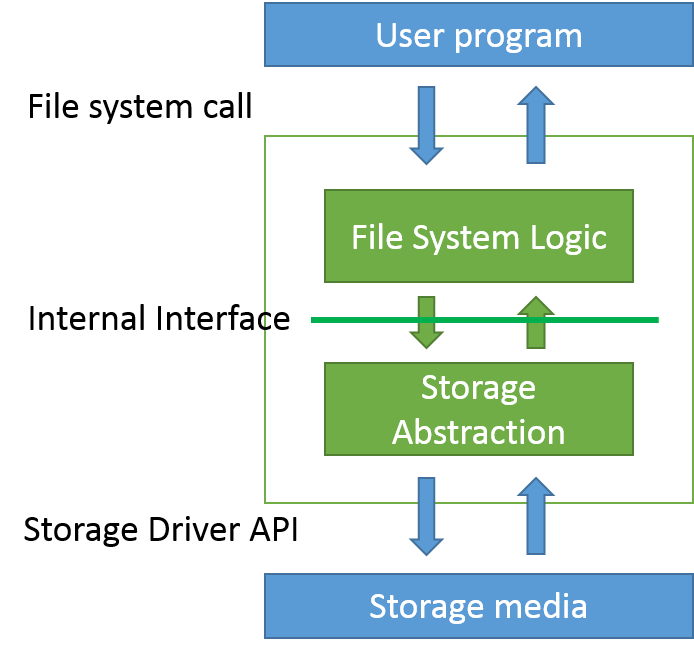
\includegraphics[width=0.5\textwidth]{Chapter-3/figs/fig8.png}
\caption{Modules of Kabi File System}
\label{fig:modules}
\end{figure}

    As shown in \fref{fig:modules}, the Kabi File System has two internal modules and an internal interface in-between. The design is for replaceable modules. The internal interface defines some primary data structures (shown in \tref{tab:data_struct}) and a set of standard operations on these data structures. The file system logic module decomposes any incoming file system call to a series of standard operations. While the storage abstraction module abstracts the underlying storage media to the primary data structures and exposes a set of method that implements the standard operations.

\begin{table}
\caption{Primary Data Structures}
\label{tab:data_struct}
\begin{center}
\begin{tabular}{ll}
\toprule
Data structures & Remark\\
\midrule
Block Node & Stores file data trunk\\
File Node & Stores the metadata of a file\\
Directory Node & Stores metadata of a directory \\
Snapshot Node & Stores metadata of a snapshot\\
\bottomrule
\end{tabular}
\end{center}
\end{table}

    The user program communicates with the file system logic module through operating system's file system APIs. Therefore, we can have different implementations of file system logic module for different file system API (e.g. FUSE, Dokan, POSIX). The storage abstraction module operates the underlying storage media through its driver, protocol or API. We can also have different implementations of storage abstraction module for different storage media (e.g. MongoDB, Volume manager, Amazon S3 service). By using this design, we can easily migrate the file system to other operating system (by changing the file system logic module) or other underlying storage media (by replacing the storage abstraction module). In our proof-of-concept implementation, the file system logic module is bind with FUSE and the storage abstraction module is written for MongoDB. 

\begin{figure}[hbtp]
\centering
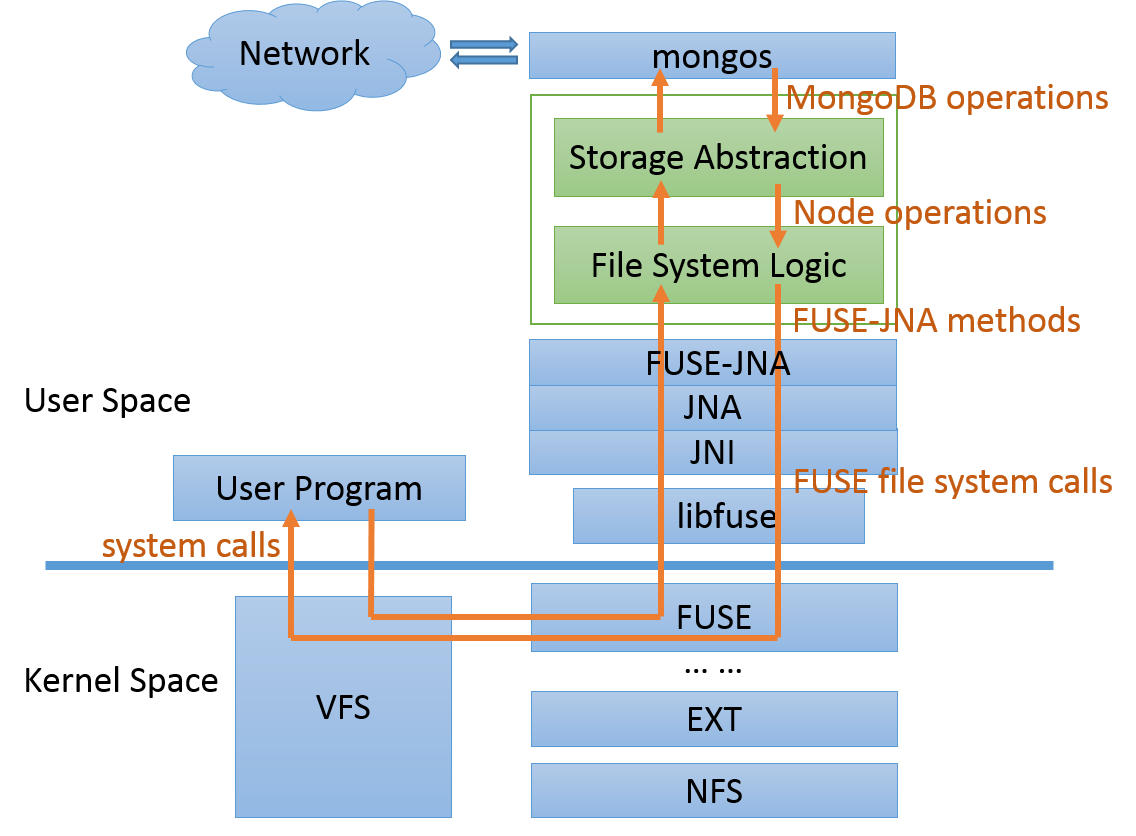
\includegraphics[width=0.8\textwidth]{Chapter-3/figs/fig1.png}
\caption{System Diagram of Kabi File System}
\label{fig:diagram}
\end{figure}

    The system diagram in \fref{fig:diagram} shows the relationship between the file system, MongoDB and operating system in this implementation. FUSE is used to connect the user program file system calls to the Kabi File System. A file system call from a user program will first be captured by VFS module in the kernel and routed to FUSE. FUSE will then pass on the file system call to the file system and pop the return value back to VFS module. On the other side, the MongoDB Java driver is used by system abstraction module to communicate with the MongoDB daemon process.

\section{File System Initialization}

    On file system initialization, parameters related to this instance of Kabi File system must be provided and be stored in a MongoDB collection. For example, the size of data block in bytes and the name of the MongoDB collection used by the file system. These parameters are immutable once the file system is established.

    On file system mount operation, the mount program requires a JSON format configuration file. The configuration file contains parameters related to this mount operation. It has three sections, which specify the FUSE options, MongoDB options, and file system client options. These parameters are important to know about the data source (such as the IP address and server status of MongoDB server), the snapshot to be mounted and the name of the MongoDB collection where the initialization parameter is written. These parameters only affect this mount on the local machine and do not have influence on the remote server.

\section{Nodes and Objects}

    Nodes are the primary data structures in the Kabi File System. A node is stored as a document in MongoDB and each type of node corresponds to a collection in MongoDB. A node can have a complex structure. A member of a node structure can be as simple as an integer but also can be as complex as an array of dictionaries. For the convenience of discussion, complex substructures will be discussed seperately. These substructures are part of the node structure and will be called ``object'' instead of ``node''. The section object and the subnode object will be discussed in this chapter and the patch object will be discussed in \cref{chap:snapshot}.

    \fref{fig:basic_entities} shows a basic view of the nodes and their relations in the Kabi File System. It consists of four nodes and an object: the block node, the directory node, the file node, the snapshot node, and the patch object. They refer to each other and form a directed acyclic graph. 

\begin{figure}[hbtp]
\centering
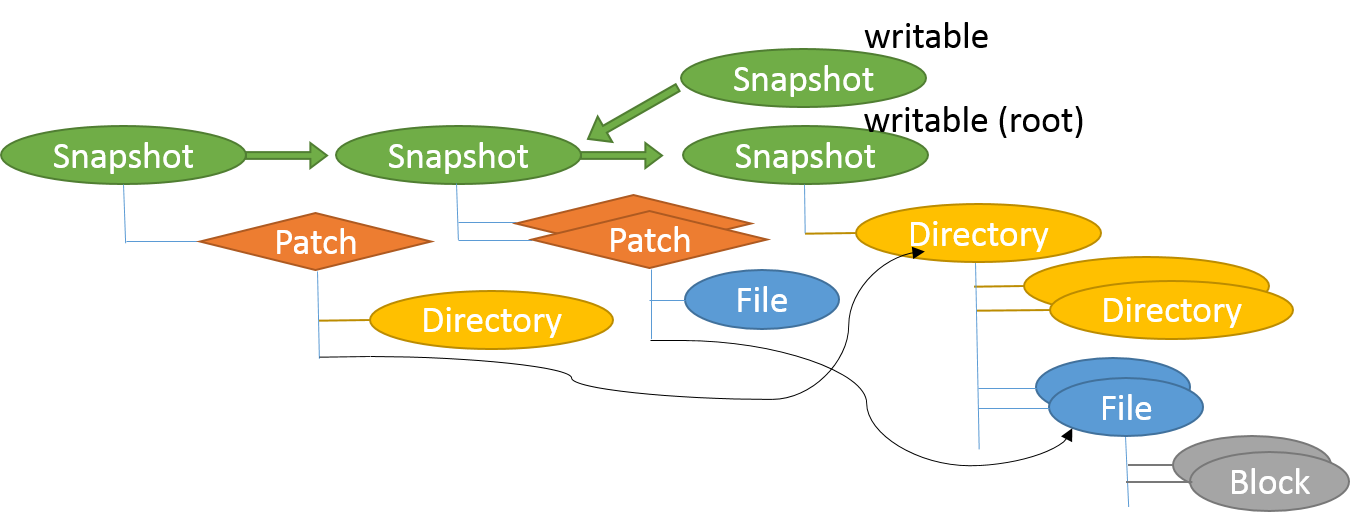
\includegraphics[width=0.9\textwidth]{Chapter-3/figs/fig2.png}
\caption{Basic Entities and Relations}
\label{fig:basic_entities}
\end{figure}

\subsection{Block nodes}

    Block node is one of the basic entities in this file system. A block node is a representation of fixed-size data. That size of data represented by the node is called representation size. The rep-size is an immutable parameter which is determined on file system initialization. Different instance of Kabi file system can have different rep-size. Although rep-size is fixed, a block node does not have to actually store that amount. If the size of data stored in block node is smaller than rep-size, when reading the block node, the Kabi file system automatically append `\textbackslash0' into the memory buffer. The fixed rep-size is to ensure that each rolling hash correspond to exact one block node since the rolling hash is a function on fixed length data. While the variable actual data length is designed to make ``truncated section'' (discussed in \cref{chap:snapshot}) more efficient. In addition to the data field, the other filed of a block node is a 128 bit hash of the byte string. This field is for deduplication and will be discussed in later section. The structure of a typical block node is shown in \tref{tab:block_fields}.

\begin{table}
\caption{Fields in Block Node}
\label{tab:block_fields}
\begin{center}
\begin{tabular}{ll}
\toprule
field & remark\\
\midrule
ID & the 128 bit SHA hash of block data\\
data & the block data\\
\bottomrule
\end{tabular}
\end{center}
\end{table}

\subsection{File node and section object}

    Each file in the Kabi File System is associated with a file node that holds the metadata of the file. In the Kabi File System, the content of the file is made up of several sections of variable length and each section is represented through a ``section object''. A file node consists of an array of section objects and other fields. Connecting the content of data section in order forms the content of the file. Each data section corresponds to exactly one block node and the block node may contribute only part of its binary data to the data section instead of its entire binary data. If only a part of the block node data is used by the data section, two integers will be specified to locate the start index and end index. This design is for reusing the block node in the snapshot system. By such design, if a block node is partly overwritten and the original block node is saved for snapshot system, we can use part of the original data to represent part of the content in file. \fref{fig:file_and_section} shows a file node that consist of 3 data sections where the first data section contributes all 4 bytes of corresponding block node data, the second section gets 2 bytes from its corresponding block node and the last section receives the first 2 bytes from its corresponding block node. The detailed structure of a file node is shown in \tref{tab:file_fields}.

\begin{figure}[hbtp]
\centering
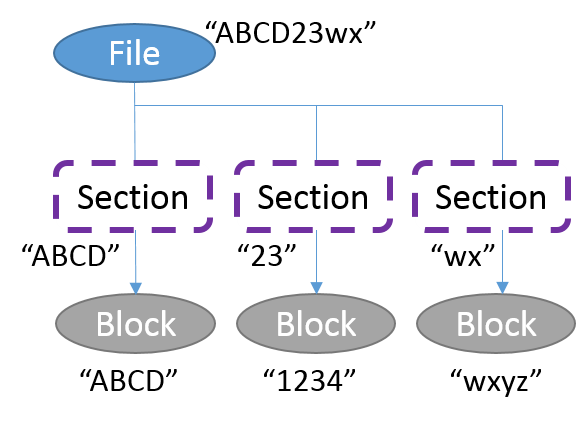
\includegraphics[width=0.5\textwidth]{Chapter-3/figs/fig7.png}
\caption{File Node, Section Object and Block Node}
\label{fig:file_and_section}
\end{figure}


\begin{table}
\caption{Fields in File Node}
\label{tab:file_fields}
\begin{center}
\begin{tabular}{ll}
\toprule
field & remark\\
\midrule
mode & access mode of the directory\\
arc & a list of Section object\\
size & size of the file\\
owner & owner of the directory\\
gowner & group owner of the directory\\
modified & timestamp of last modification\\
\bottomrule
\end{tabular}
\end{center}
\end{table}

    As mentioned above, a file node has an array of section object. Each section object is a substructure of file node and represents a section of file data. It consists of three fields as shown in \tref{tab:section_fields}: an object ID referring to the associate block node, an integer value specifies the number of omitted leading bytes, and another integer value specifying the index of last byte in block node. In the example shown in \fref{fig:section_and_block}, for the second block, the number of omitted leading bytes is 1, and the index of the last byte in block is 5.

\begin{figure}[hbtp]
\centering
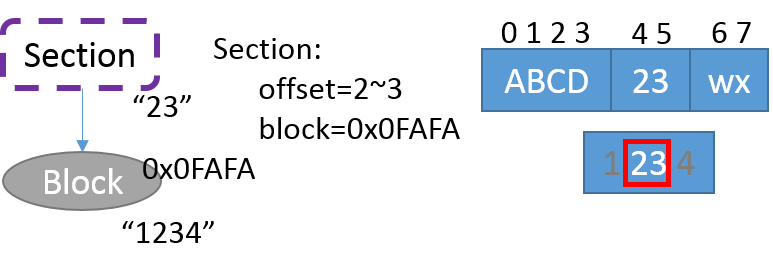
\includegraphics[width=0.9\textwidth]{Chapter-3/figs/fig9.png}
\caption{Section Object and Block Node}
\label{fig:section_and_block}
\end{figure}

\begin{table}
\caption{Fields in Section Object}
\label{tab:section_fields}
\begin{center}
\begin{tabular}{ll}
\toprule
field & remark\\
\midrule
ID & ID of corresponding block\\
roll & the 32 bit rolling hash of block data\\
omit & specify how many leading bytes in block will be omitted\\
offset & the offset of last byte in this section\\
\bottomrule
\end{tabular}
\end{center}
\end{table}

    The size field stores an integer value, representing the size of this file in bytes. When reading the file, `\textbackslash0' padding will be append to the end of files in read buffer if the value in the ``size'' field exceed the total number of bytes in its data sections. On the contrary, if the total number of bytes in data sections exceeds the value of the ``size'' field, data will be truncated and the data exceeds the size will not be noticed by end user. This design allows faster creation and truncate operation to a file.

\subsection{Directory node and subnode object}

     A directory node corresponds to a directory in the file system. Directory nodes share similar structures with the file node, it also consists of fields that store the metadata and an array of subnode objects. The subnode object is similar to the section object in file node. A subnode object corresponds to an ``item'' under the directory. A subnode object contains a reference to the ``item'' and a string represents the display name of the ``item''. Depending on the type of node that a subnode object is referencing, the ``item'' can be a file under the directory or a sub directory.

\begin{table}
\caption{Fields in Directory Node}
\label{tab:dir_fields}
\begin{center}
\begin{tabular}{ll}
\toprule
field & remark\\
\midrule
mode & access mode of the directory\\
arc & a list of Subnode object\\
owner & owner of the directory\\
gowner & group owner of the directory\\
modified & timestamp for last modification\\
\bottomrule
\end{tabular}
\end{center}
\end{table}

\begin{table}
\caption{Fields in Subnode Object}
\label{tab:subnode_fields}
\begin{center}
\begin{tabular}{ll}
\toprule
field & remark\\
\midrule
name & display name of the file or subdirectory\\
ID & ID of the file or subdirectory\\
\bottomrule
\end{tabular}
\end{center}
\end{table}

    Other important data structures are snapshot node and patch object. These two structures are related to the snapshot system and will be discussed in \cref{chap:snapshot}.

\section{File System Operations}

    The file system logic module decomposes the FUSE file system calls to standard node operations defined by the internal interface. Most of the FUSE file system calls have been implemented in the Kabi File System, some of those important calls include access(), getattr(), read(), write(), rmdir(), unlink(), mkdir(), truncate(), flush(), open() and release(). Related node operations are addDirNode2db(), addFileNode2db(), addDataNode2db() and patch(). The former three methods write a node object into the database as a new node. The patch() method replaces an existing node with its new version.

\subsection{Read operations}

    Three important read file system calls are access(), getattr(), and read(). The access() function tests the existence and permission settings of a file or directory in the file system. getattr() returns the meta information about a file or directory. The read() function reads and returns binary data of given length starting at a specified offset.

    The first step of a read operation is finding the target file or directory node by its path. In order to do so, the file system parses the given path and finds all corresponding nodes on the path in order from root directory to the target. The file system will start with the root directory, continue traversing subnode list and find directories on the path one by one until the algorithm hit the target or find it nowhere.

    This strategy is generally not satisfactory. Because it may introduce a performance bottleneck into the file system read operation when the target lies deep in the directory tree. In such case, a simple access() call will be mapped to a sequence of database queries on directory nodes. To solve this issue, a cache that stores the path and corresponding node ID is introduced. It can be a cache in memory when the file system is mounted locally with FUSE's single thread option or a cache in MongoDB when multiple threads or client for consistency. With the help of the path cache, the file system no longer needs to traverse and find every directory node on the path.

    The path cache is a move-to-front dictionary \cite{mtf} which maps a path string to a integer which represents an ID of directory node or a file node. The cache has a fixed capacity and assumes temporal locality in the access pattern. It uses move-to-front algorithm to keep the ID of frequently accessed hot item in the cache and remove those cold items that have not been accessed for long. The cache also assumes spatial locality: when accessing a file or directory, not only the ID of corresponding file or directory itself is cached but all directories on the path, i.e., its parent and ancestor directories, also go into the cache. Thus, when touching contents under the same directory later, the file system can directly find its parent node in cache.

    Once the file node is retrieved, reading the file become straight forward. The file system will traverse the section object array to find the ID of block node associated with the read call. It will then calculate the begin and end index of the bytes of the block content that will be copied to read buffer. At last the file system will query MongoDB for block nodes and copy requested data to buffer.

\subsection{Write operations}

\begin{figure}[hbtp]
\centering
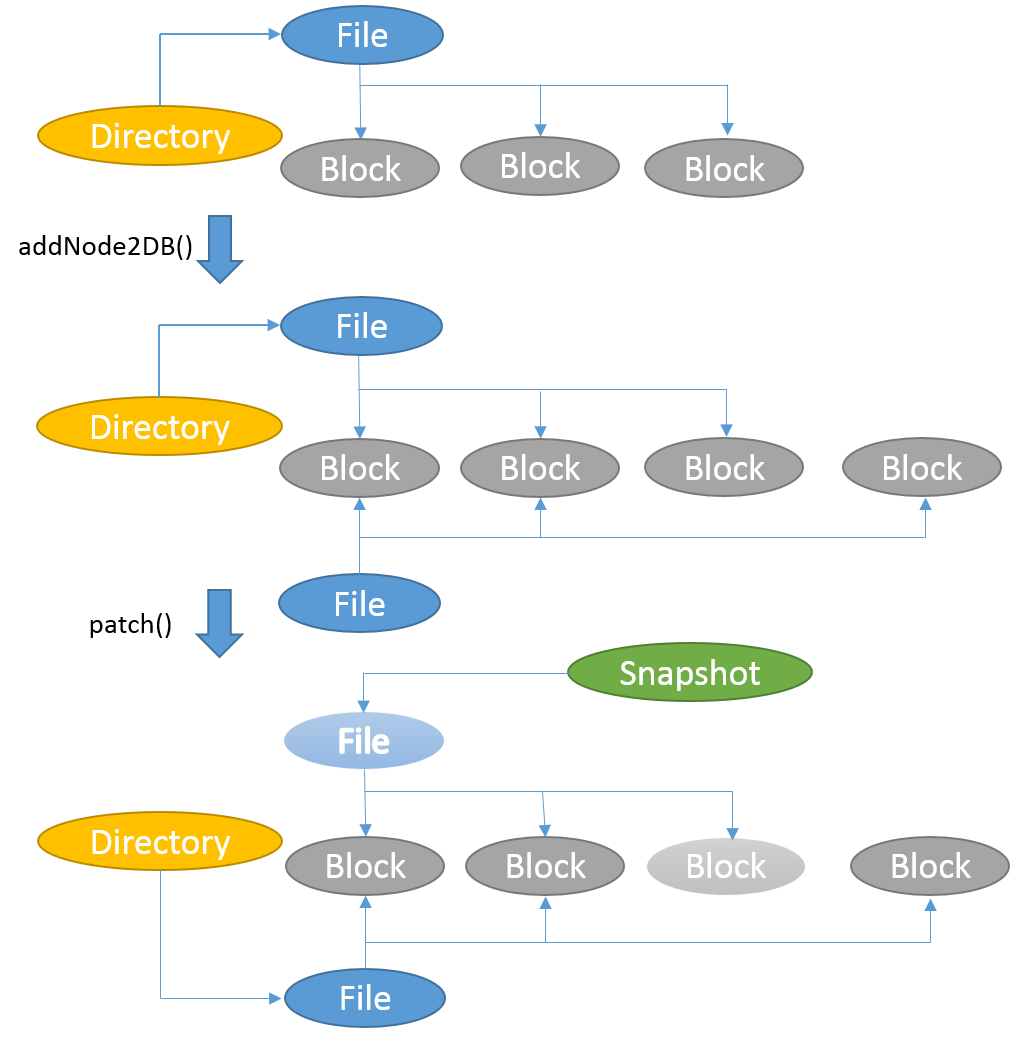
\includegraphics[width=0.8\textwidth]{Chapter-3/figs/fig10.png}
\caption{Copy-on-Write}
\label{fig:cow}
\end{figure}

    The Kabi File System write files on file close or explicit flush. It uses write() call to write data into a file from some offset. Other write calls like chmod(), chown(), mkdir(), unlink() and rmdir() change the meta information of a directory or file.

    Block nodes are designed to be immutable. File nodes and directory nodes use copy-on-write strategy when an overwrite is requested. So, when an overwrite to file node or directory node is requested, the file system will make a local copy of the node and apply the modification to this local copy. The file system will then upload that copy to remote and attach it to its parent directory replacing the original node as shown in the \fref{fig:cow}. In this way, the old version of the node is saved for snapshot and read operation will not accidentally read in a node that is in an incomplete state. As shown in \fref{fig:cow}, during this process, we use addNode2DB() operation to add a new node and use the patch() method to replace the old version with this new node.

	When writing a file, the write request will not immediately flush data into persistent storage. Instead, the data will be written into a local write buffer. Data in write buffer will be merged and subsequent write will overwrite previous buffered data when there is an overlap. When the file system receives a close() call or an explicit flush() request, data in buffer will be truncated into blocks and uploaded to remote servers. The content in local buffer may lost due to a system failure, but user can always use a fsync() or fdatasync() as suggested in POSIX standard to flush important data to remote. The flush process is atomic, guaranteed by MongoDB. 

\begin{figure}[hbtp]
\centering
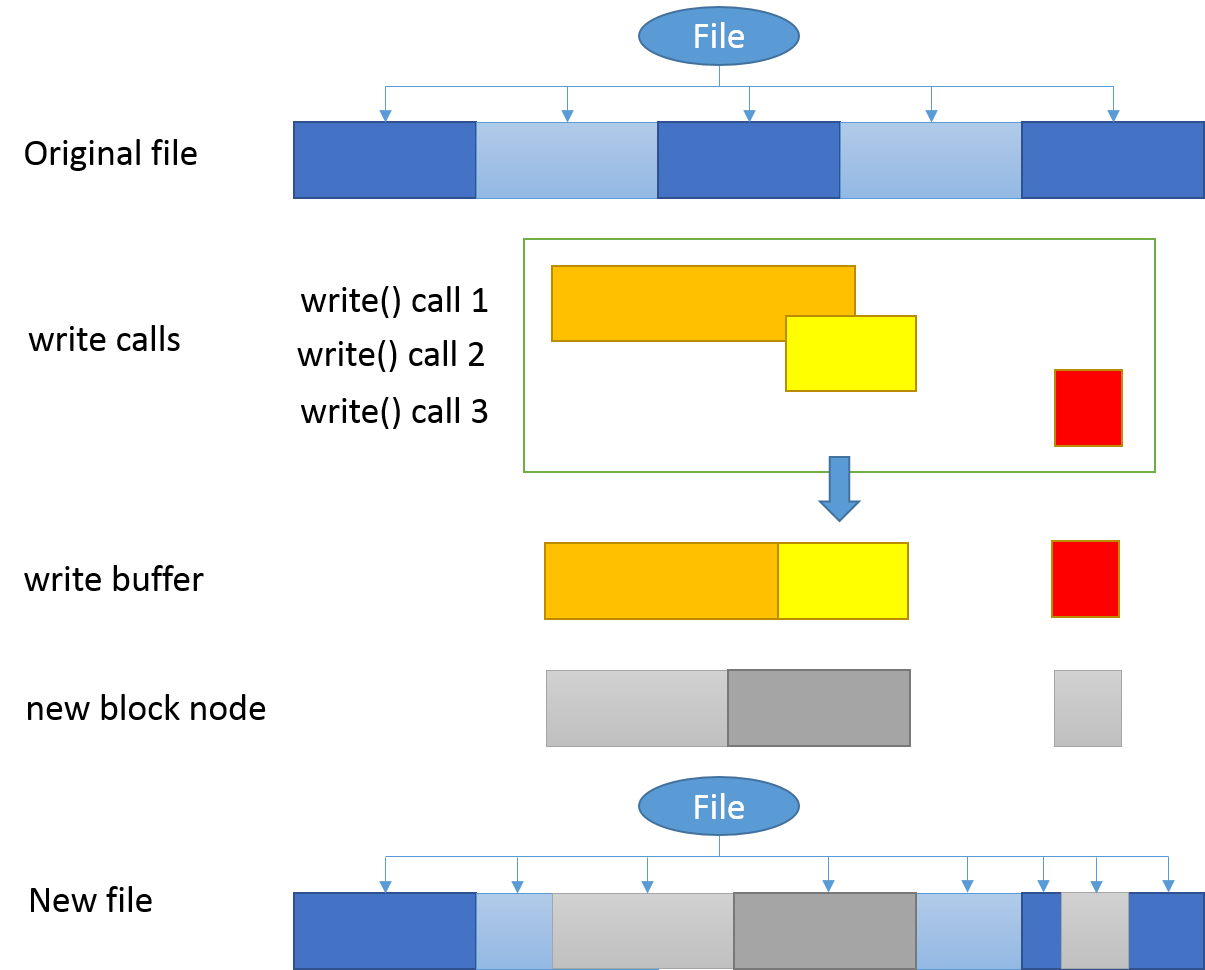
\includegraphics[width=0.8\textwidth]{Chapter-3/figs/fig11.png}
\caption{Write Buffer}
\label{fig:buffer}
\end{figure}

    During a flush, a data section (section object) may be unaffected, partly overwritten or entirely overwritten. Block node will be detached from the file if its corresponding data section has been entirely overwritten. The data section object will be truncated if this section is partly overwritten. If a section is truncated, the start offset and end offset will be updated to reflect the change while the block node remain the same. The \fref{fig:buffer} shows the routine to write a file.

    Compared to the traditional copy-on-write snapshot file system which copies and overwrites the entire block whenever there is a byte change, this design can make use of the old block. Because the old block will be kept for snapshot, reusing it in current view may save some storage.

    However, there is a tradeoff between these savings and the overhead of such design. Each data section object requires 224 bit storage to store its SHA hash, rolling hash and begin/end indexes, each block node requires 128 bit to store its SHA ID. There're many cases where this overhead is worthy. In the extreme case, if we overwrite 2 bytes on the boundary of two blocks right after a snapshot is taken, two new blocks will be created in classic copy-on-write snapshot system but only a 2-byte block will be added in our design. With a block size of 2,048 bytes and a file size of 20,480 byte, the saving in this case is 3,798 bytes.

\subsection{Consistency}

    Maintaining consistency is an important task for file system. During a write call, the file system may enter an incomplete state before the write call successfully returns. A file system should prevent a read call from reaching the incomplete state to keep consistency. There are many ways to keep a system consistent. Some of the file systems use lock to prevent a read operation when the file system is processing a write call. In our implementation, we use atomic update to prevent the incomplete state.

\begin{figure}[hbtp]
\centering
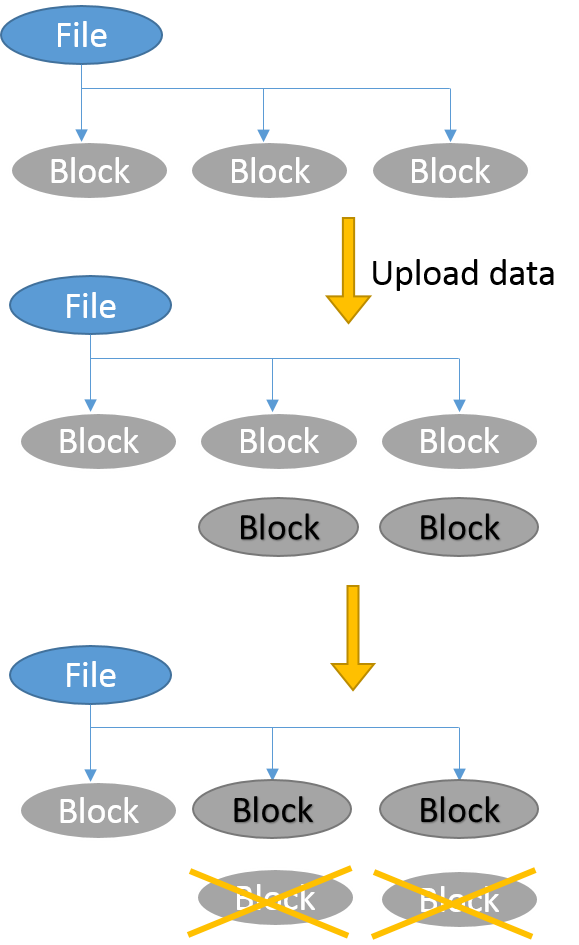
\includegraphics[width=0.8\textwidth]{Chapter-3/figs/fig27.png}
\caption{Consistency - within a snapshot}
\label{fig:consist1}
\end{figure}

\begin{figure}[hbtp]
\centering
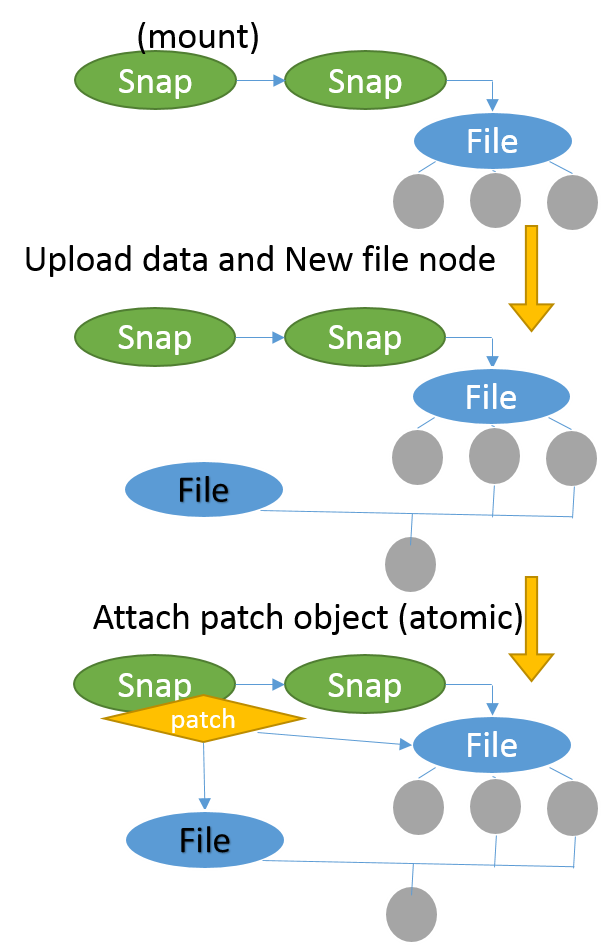
\includegraphics[width=0.8\textwidth]{Chapter-3/figs/fig28.png}
\caption{Consistency - cross snapshots}
\label{fig:consist2}
\end{figure}

    \fref{fig:consist1} and \fref{fig:consist2} demonstrates how we prevent incomplete state. The write process can be divided into two steps. The first step is upload, where we upload the new data node and the new version of metadata node that is going to be affected. In this step, read operations may come in at any time and observe the old content because all new nodes are not connected to the directed graph and all old nodes haven't been modified. The second step is atomic update. This step is always atomic, guaranteed by MongoDB. In this step, the file system will change affected reference from referring the old node to new node. When a write operation only affects one snapshot. The file system will directly replace the old node with new node by update referring reference as shown in \fref{fig:consist1}. When a write operation affects more than one snapshot, the file system will upload a patch object to replace the old node with new node and then attach the object to the snapshot node in step 2.

\subsection{Deduplication}

    In a copy-on-write file system, block nodes are immutable thus there's no in-place modification to block nodes. Therefore, in most cases, making a change to the file system means creation of new block node. This is an expensive operation as it requires storage space on remote and all data must be transferred to remote.
    
    We found that not all block node creations are necessary. Consider the following scenario, when some user program is trying to create a copy of a file, the program will read in all data from the file to a buffer and then write the data in the buffer to another newly created file. As a result, the file system will experience a series of read() and write() function call, not aware that these function calls are related. File system has no way to know that the block node it is going to write already exists in the file system and can be reused.

    By using SHA hash as the block node ID, it is possible to find and eliminate blocks that contain duplicate data. Before a block of binary data is uploaded, the file system will query the database with its SHA hash. If a instance with same ID is found, the file system will stop unloading the block node but directly return the ID of existing node with same hash value. In this way, the file system not only can perform a copy operation efficiently but also save space for duplicate blocks. 

\section{Conclusion}

    In this chapter, we presented a design of distributed file system with replaceable modules. We demonstrated the overview of the file system, some detailed design choices like the cache and deduplicate feature.

